%%%%%%%%%%%%%%%%%%%%%%%%%%%%%%%%%%%%%%%%%
% Short Sectioned Assignment LaTeX Template Version 1.0 (5/5/12)
% This template has been downloaded from: http://www.LaTeXTemplates.com
% Original author:  Frits Wenneker (http://www.howtotex.com)
% License: CC BY-NC-SA 3.0 (http://creativecommons.org/licenses/by-nc-sa/3.0/)
%%%%%%%%%%%%%%%%%%%%%%%%%%%%%%%%%%%%%%%%%

%----------------------------------------------------------------------------------------
%	PACKAGES AND OTHER DOCUMENT CONFIGURATIONS
%----------------------------------------------------------------------------------------

\documentclass[paper=a4, fontsize=11pt]{scrartcl} % A4 paper and 11pt font size

% ---- Entrada y salida de texto -----

\usepackage{hyperref}
\usepackage{varioref}
\usepackage[T1]{fontenc} % Use 8-bit encoding that has 256 glyphs
\usepackage[utf8]{inputenc}
%\usepackage{fourier} % Use the Adobe Utopia font for the document - comment this line to return to the LaTeX default

% ---- Idioma --------

\usepackage[spanish, es-tabla]{babel} % Selecciona el español para palabras introducidas automáticamente, p.ej. "septiembre" en la fecha y especifica que se use la palabra Tabla en vez de Cuadro

% ---- Otros paquetes ----

\usepackage{amsmath,amsfonts,amsthm} % Math packages
%\usepackage{graphics,graphicx, floatrow} %para incluir imágenes y notas en las imágenes
\usepackage{graphics,graphicx, float} %para incluir imágenes y colocarlas

% Para hacer tablas comlejas
%\usepackage{multirow}
%\usepackage{threeparttable}

%\usepackage{sectsty} % Allows customizing section commands
%\allsectionsfont{\centering \normalfont\scshape} % Make all sections centered, the default font and small caps

\usepackage{fancyhdr} % Custom headers and footers
\pagestyle{fancyplain} % Makes all pages in the document conform to the custom headers and footers
\fancyhead{} % No page header - if you want one, create it in the same way as the footers below
\fancyfoot[L]{} % Empty left footer
\fancyfoot[C]{} % Empty center footer
\fancyfoot[R]{\thepage} % Page numbering for right footer
\renewcommand{\headrulewidth}{0pt} % Remove header underlines
\renewcommand{\footrulewidth}{0pt} % Remove footer underlines
\setlength{\headheight}{13.6pt} % Customize the height of the header

\numberwithin{equation}{section} % Number equations within sections (i.e. 1.1, 1.2, 2.1, 2.2 instead of 1, 2, 3, 4)
\numberwithin{figure}{section} % Number figures within sections (i.e. 1.1, 1.2, 2.1, 2.2 instead of 1, 2, 3, 4)
\numberwithin{table}{section} % Number tables within sections (i.e. 1.1, 1.2, 2.1, 2.2 instead of 1, 2, 3, 4)

\setlength\parindent{0pt} % Removes all indentation from paragraphs - comment this line for an assignment with lots of text

\newcommand{\horrule}[1]{\rule{\linewidth}{#1}} % Create horizontal rule command with 1 argument of height


%----------------------------------------------------------------------------------------
%	TÍTULO Y DATOS DEL ALUMNO
%----------------------------------------------------------------------------------------

\title{	
\normalfont \normalsize 
\textsc{{\bf Ingeniería de Servidores (2015-2016)} \\ Grado en Ingeniería Informática \\ Universidad de Granada} \\ [25pt] % Your university, school and/or department name(s)
\horrule{0.5pt} \\[0.4cm] % Thin top horizontal rule
\huge Cuestiones Opcionales \\ % The assignment title
\horrule{2pt} \\[0.5cm] % Thick bottom horizontal rule
}

\author{Francisco Carrillo Pérez} % Nombre y apellidos

\date{\normalsize\today} % Incluye la fecha actual

%----------------------------------------------------------------------------------------
% DOCUMENTO
%----------------------------------------------------------------------------------------

\begin{document}

\maketitle % Muestra el Título

\newpage %inserta un salto de página

\tableofcontents % para generar el índice de contenidos

\listoffigures

\listoftables

\newpage

%%%%%%%%%%%%%%%%%%%%%%%%%%%%%%%%%%%%%%%%%%%%%%%%%%%%
% CUESTIÓN 1
%%%%%%%%%%%%%%%%%%%%%%%%%%%%%%%%%%%%%%%%%%%%%%%%%%%%

\section{Cuestion opcional 1: ¿Qué gestores utiliza OpenSuse?}

Dentro de la documentación de OpenSuse \cite{gestorpaquetesopen} podemos observar qué el gestor de paquetes de forma gráfica utiliza YaST \cite{yast} pero para la línea de comandos utiliza Zypper \cite{zipper}.

%%%%%%%%%%%%%%%%%%%%%%%%%%%%%%%%%%%%%%%%%%%%%%%%%%%%
% CUESTIÓN 2
%%%%%%%%%%%%%%%%%%%%%%%%%%%%%%%%%%%%%%%%%%%%%%%%%%%%

\section{Cuestión opcional 6: Muestre un ejemplo de uso para awk}

Vamos a utilizar el siguiente ejemplo \cite{awk}:

\begin{itemize}
	\item Primero creamos un archivo para poder tratarlo con awk. Para ello utilizamos el comando: \textbf{ls -l > inputfile.txt}. Podemos observar como queda en la Figura \ref{figura1}.
	\item Ahora vamos a imprimir la primera columna. Para ello ejecutamos el comando: \textbf{awk '{print \$1}' inputfile.txt}. Podemos observar el resultado en la Figura \ref{figura2}.
	\item Otro ejemplo sería imprimir la segunda columna. Para ello ejecutamos el comando: \textbf{awk '{print \$2}' inputfile.txt}. Podemos observar el resultado en la Figura \ref{figura3}.
\end{itemize}

\begin{figure}[H] %con el [H] le obligamos a situar aquí la figura
	\centering
	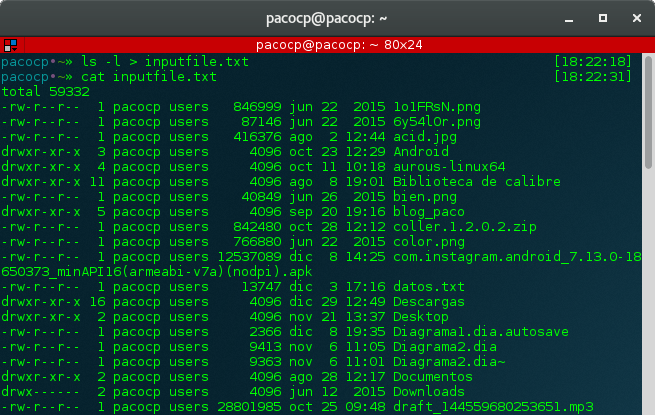
\includegraphics[scale=0.5]{figuras/figura1.png}  %el parámetro scale permite agrandar o achicar la imagen. En el nombre de archivo puede especificar directorios

	
	\caption{Resultado al ejecutar \textbf{ls -l > inputfile.txt}}
	\label{figura1}
\end{figure}

\begin{figure}[H] %con el [H] le obligamos a situar aquí la figura
	\centering
	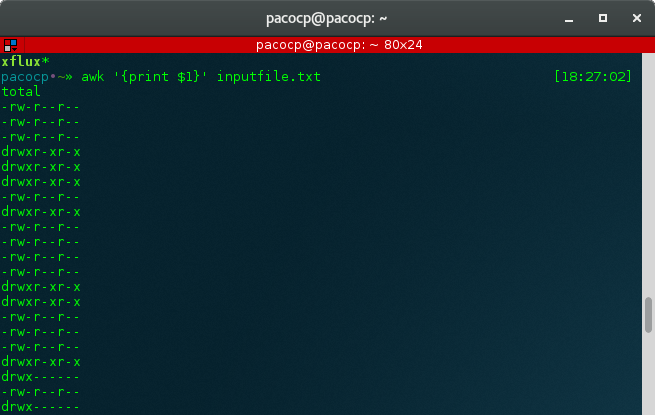
\includegraphics[scale=0.5]{figuras/figura2.png}  %el parámetro scale permite agrandar o achicar la imagen. En el nombre de archivo puede especificar directorios
	
	
	\caption{Resultado al ejecutar \textbf{awk '{print \$1}' inputfile.txt}}
	\label{figura2}
\end{figure}

\begin{figure}[H] %con el [H] le obligamos a situar aquí la figura
	\centering
	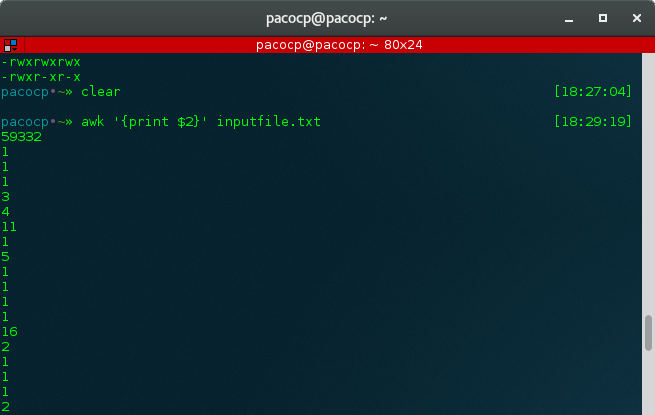
\includegraphics[scale=0.5]{figuras/figura3.png}  %el parámetro scale permite agrandar o achicar la imagen. En el nombre de archivo puede especificar directorios
	
	
	\caption{Resultado al ejecutar \textbf{awk '{print \$2}' inputfile.txt}}
	\label{figura3}
\end{figure}
%%%%%%%%%%%%%%%%%%%%%%%%%%%%%%%%%%%%%%%%%%%%%%%%%%%%
% CUESTIÓN 3
%%%%%%%%%%%%%%%%%%%%%%%%%%%%%%%%%%%%%%%%%%%%%%%%%%%%

%Práctica 2

\section{Cuestión opcional 3: Instale el servicio y pruebe su funcionamiento.}

Voy a seguir el tutorial encontrado en la siguiente página de DigitalOcean \cite{fail2ban}.\\
Para instalarlo usamos el comando: \textbf{sudo apt-get install fail2ban}, como podemos observar en la Figura \ref{figura11}.\\

Ahora vamos a compiar el archivo \textbf{jail.conf} a la dirección \textbf{/etc/fail2ban/jail.local} para no tocar el jail.conf, podemos observarlo en la Figura \ref{figura12}. Y activamos el servicio con \textbf{sudo service fail2ban start}, como podemos observar en la Figura 
\ref{figura13}.

Ahora desde mi máquina voy a fallar la conexión ssh varias veces para que me meta en la lista negra. Podemos observarlo en a Figura \ref{figura27}, haciendo uso del comando \textbf{sudo iptables -S}.

\begin{figure}[H] %con el [H] le obligamos a situar aquí la figura
	\centering
	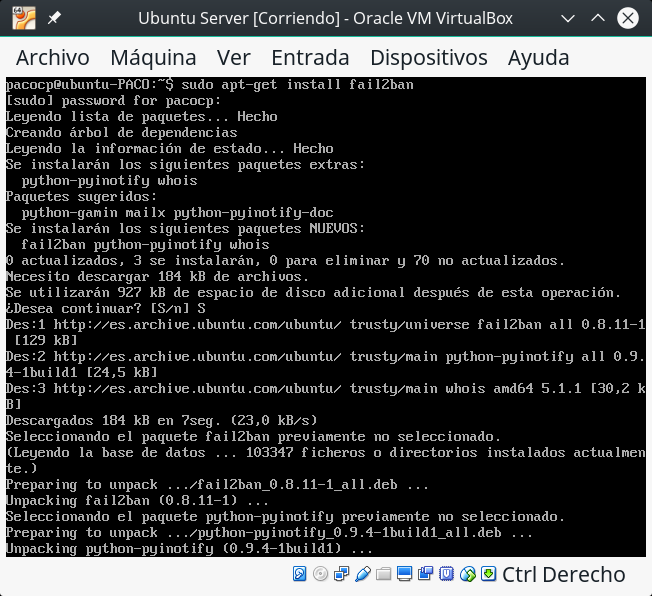
\includegraphics[scale=0.5]{figuras/figura11.png}  %el parámetro scale permite agrandar o achicar la imagen. En el nombre de archivo puede especificar directorios
	
	
	\caption{Resultado de ejecutar el comando \textbf{sudo apt-get install fail2ban}}
	\label{figura11}
\end{figure}

\begin{figure}[H] %con el [H] le obligamos a situar aquí la figura
	\centering
	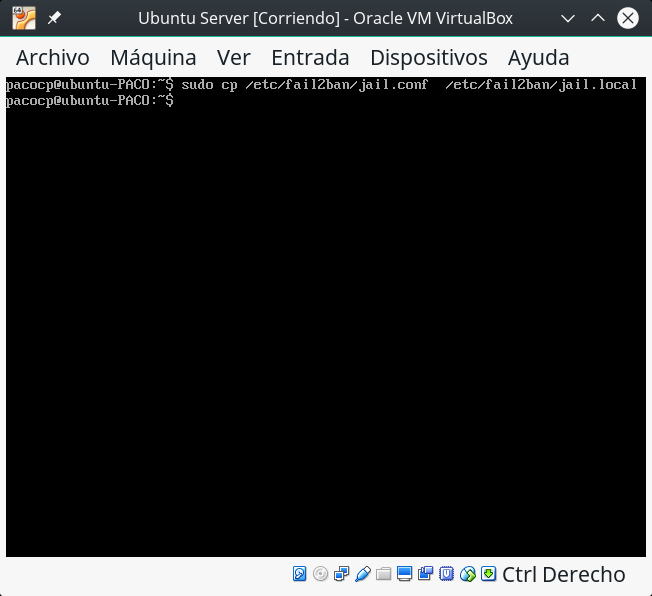
\includegraphics[scale=0.5]{figuras/figura12.png}  %el parámetro scale permite agrandar o achicar la imagen. En el nombre de archivo puede especificar directorios
	
	
	\caption{Resultado de ejecutar el comando \textbf{sudo cp /etc/fail2ban/jail.conf /etc/fail2ban/jail.local}}
	\label{figura12}
\end{figure}

\begin{figure}[H] %con el [H] le obligamos a situar aquí la figura
	\centering
	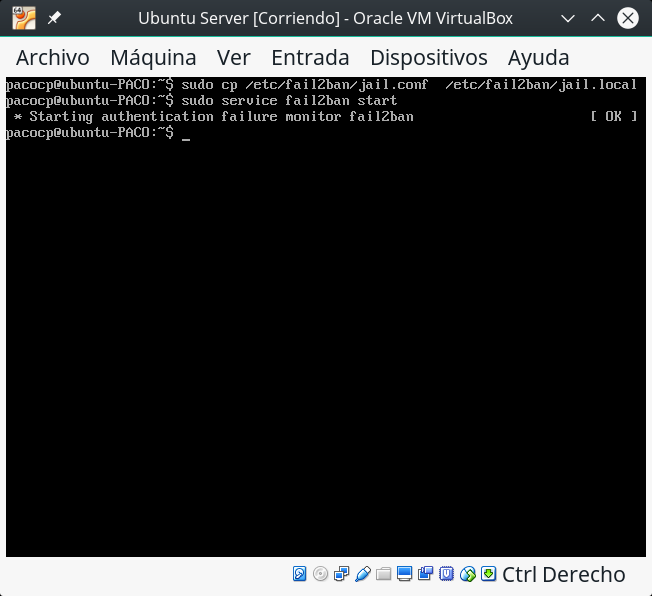
\includegraphics[scale=0.5]{figuras/figura13.png}  %el parámetro scale permite agrandar o achicar la imagen. En el nombre de archivo puede especificar directorios
	
	
	\caption{Resultado de ejecutar el comando \textbf{sudo service fail2ban start}}
	\label{figura13}
\end{figure}

\begin{figure}[H] %con el [H] le obligamos a situar aquí la figura
	\centering
	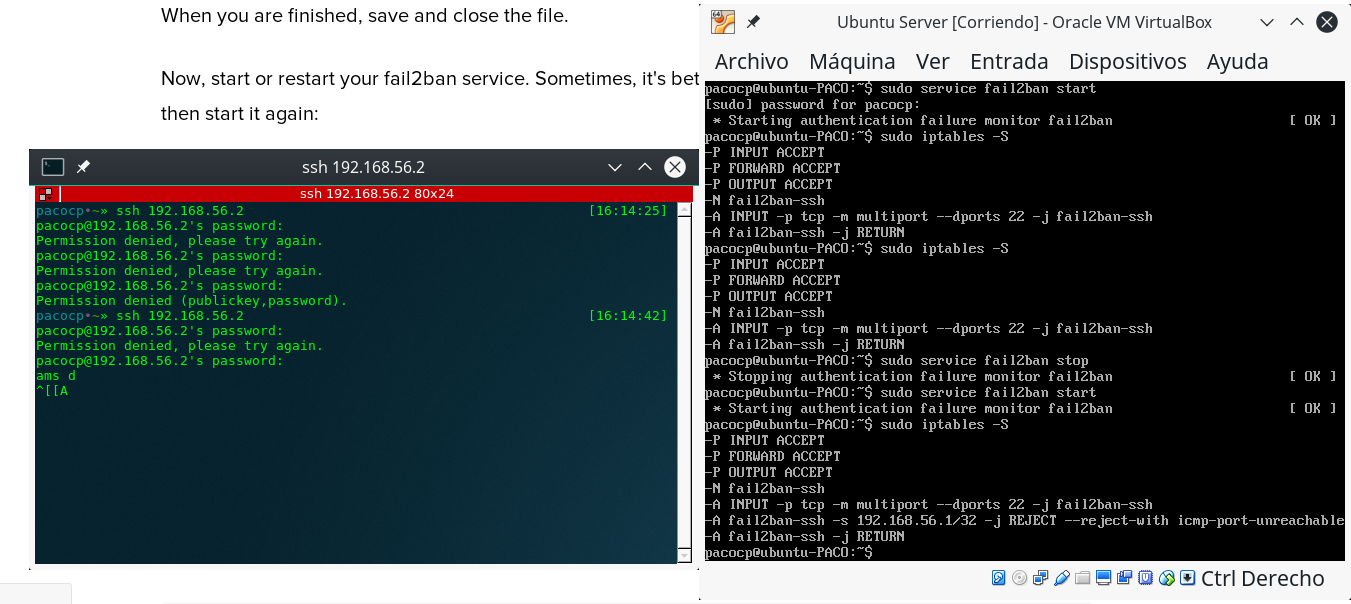
\includegraphics[scale=0.25]{figuras/figura25.png}  %el parámetro scale permite agrandar o achicar la imagen. En el nombre de archivo puede especificar directorios
	
	
	\caption{Mete mi ip en al lista negra. Podemos observarlo con el comando \textbf{sudo iptables -S}}
	\label{figura25}
\end{figure}

%%%%%%%%%%%%%%%%%%%%%%%%%%%%%%%%%%%%%%%%%%%%%%%%%%%%
% CUESTIÓN 4
%%%%%%%%%%%%%%%%%%%%%%%%%%%%%%%%%%%%%%%%%%%%%%%%%%%%

%Práctica 4

\section{Cuestión opcional 3: Lea el artículo y elabore un breve resumen.}

Lo que nos cuenta el siguiente artículo \cite{articulo}, es que van a comparar dos benchmarks como son JMeter y Garling, ambos los ofrecen en su plataforma.\\
Para ello van a crear un sitio web com  nginx, ya que necesitan que el sitio se comporte como un servidor de aplicaciones, es decir, que responda a los HTTP GETs y además a los HTTP POSTs mientras sirve contenido estático y dinámico. Tunearon el kernel del sistema operativo y la red TCP y colocaron 4 CPUs virtuales y 15 GB de RAM para asegurar que no se produjeran cuellos de botella.\\

Cuentan lo que es Flood.io y explican lo que es un nodo, y cuenta las opciones para la máquina virtual de java JVM.\\
A continuación, cuentan en el escenario en el que van a comprar las dos que consiste en:
\begin{itemize}
	\item \textbf{20 \%} de transacciones lentas en aproximadamente 3.5 s.
	\item \textbf{40 \%} de transacciones haciendo peticiones condicionales a una fuente caché en menos de 10 ms.
	\item \textbf{30 \%} de transacciones trayendo de una fuente de no caché en aproximadamente 2 s.
	\item \textbf{10 \%} de transacciones  a una fuente lenta en aproximadamente 4 s.
\end{itemize}

La concurrencia que van a usar es de 10.000 usuarios, con 30.000 peticiones por minuto y 20 minutos de duración.\\
Como conclusión,obtienendo los resultados resaltan que son bastante parecidos, y que no hay mucha diferencia entre ambas máquinas. Podemos verlos en la Figura \ref{figura28}.

\begin{figure}[H] %con el [H] le obligamos a situar aquí la figura
	\centering
	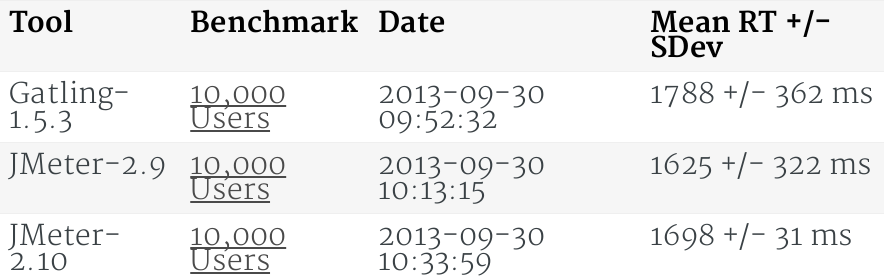
\includegraphics[scale=0.5]{figuras/figura28.png}  %el parámetro scale permite agrandar o achicar la imagen. En el nombre de archivo puede especificar directorios
	
	
	\caption{Resultados que obtiene la empresa Flood.io \cite{articulo} al realizar la comparación entre JMeter y Garling}
	\label{figura28}
\end{figure}


%%%%%%%%%%%%%%%%%%%%%%%%%%%%%%%%%%%%%%%%%%%%%%%%%%%%
% CUESTIÓN 5
%%%%%%%%%%%%%%%%%%%%%%%%%%%%%%%%%%%%%%%%%%%%%%%%%%%%

%Práctica 1

\section{Cuestión Opcional 1: Muestre (con capturas de pantalla) cómo ha comprobado que el RAID1 funciona.}

Primero vamos a ver que tenemos los dos RAID con el comando \textbf{lsblk}, podemos observalo en la Figura \ref{figura4}.\\
Ahora vamos a poner el RAID0 en faulty con el comando: \textbf{sudo mdadm --manage --set-faulty /dev/md0 /dev/sda1}, como podemos observar en la Figura \ref{figura5}\\
Para comprobar que el bloque está en faulty podemos verlo con el comando: \textbf{sudo mdadm --detail /dev/md0}, como podemos observar en la Figura \ref{figura6}\\
Ahora apagamos la máquina, y vemos si sigue arrancando.\\
Y podemos comprobar cómo sigue arrancando la máquina, por lo que funciona, como podemos observar en las Figuras \ref{figura8} y \ref{figura10}.

\begin{figure}[H] %con el [H] le obligamos a situar aquí la figura
	\centering
	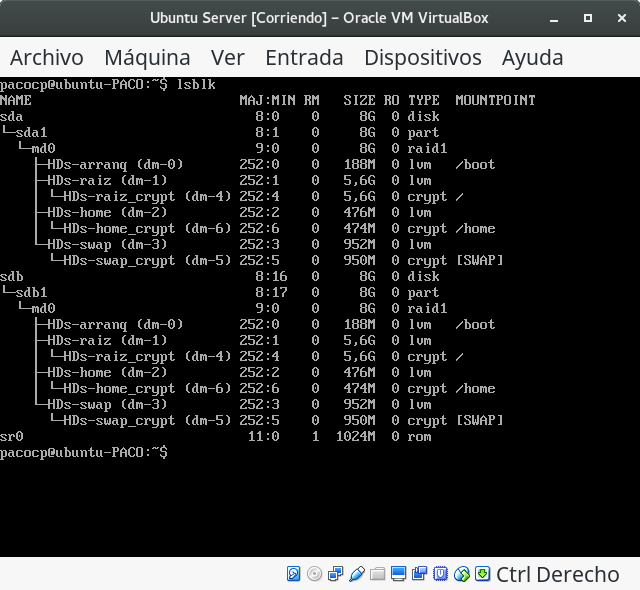
\includegraphics[scale=0.5]{figuras/figura4.png}  %el parámetro scale permite agrandar o achicar la imagen. En el nombre de archivo puede especificar directorios
	
	
	\caption{Resultado al ejecutar \textbf{lsblk}}
	\label{figura4}
\end{figure}

\begin{figure}[H] %con el [H] le obligamos a situar aquí la figura
	\centering
	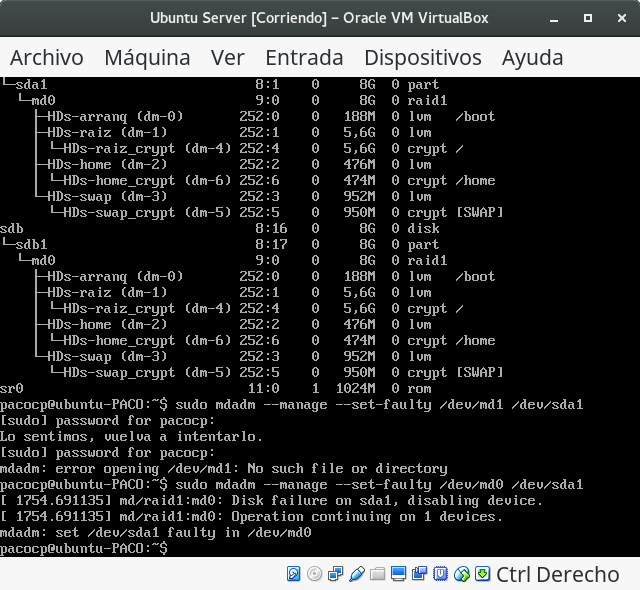
\includegraphics[scale=0.5]{figuras/figura5.png}  %el parámetro scale permite agrandar o achicar la imagen. En el nombre de archivo puede especificar directorios
	
	
	\caption{Resultado al ejecutar \textbf{sudo mdadm --manage --set-faulty /dev/md0 /dev/sda1}}
	\label{figura5}
\end{figure}

\begin{figure}[H] %con el [H] le obligamos a situar aquí la figura
	\centering
	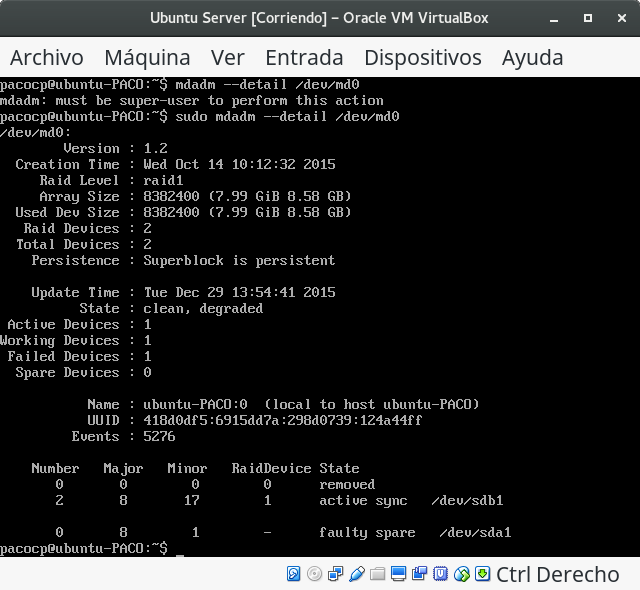
\includegraphics[scale=0.5]{figuras/figura6.png}  %el parámetro scale permite agrandar o achicar la imagen. En el nombre de archivo puede especificar directorios
	
	
	\caption{Resultado al ejecutar \textbf{sudo mdadm --detail /dev/md0}}
	\label{figura6}
\end{figure}

\begin{figure}[H] %con el [H] le obligamos a situar aquí la figura
	\centering
	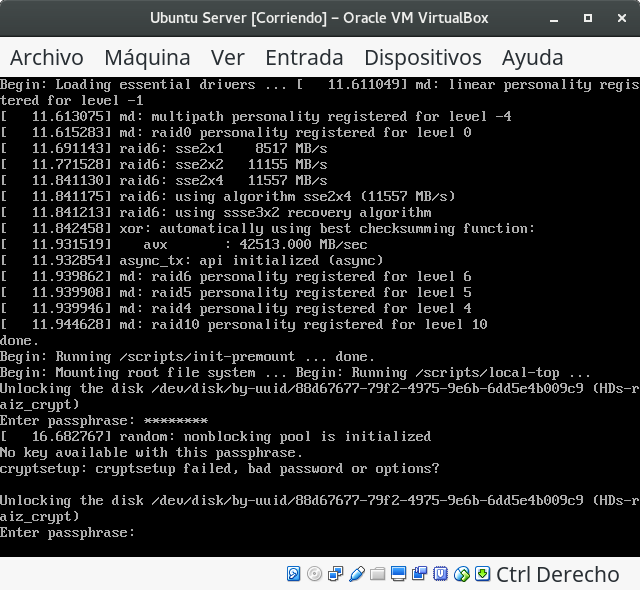
\includegraphics[scale=0.5]{figuras/figura8.png}  %el parámetro scale permite agrandar o achicar la imagen. En el nombre de archivo puede especificar directorios
	
	
	\caption{Podemos observar cómo la máquina sigue arrancando}
	\label{figura8}
\end{figure}

\begin{figure}[H] %con el [H] le obligamos a situar aquí la figura
	\centering
	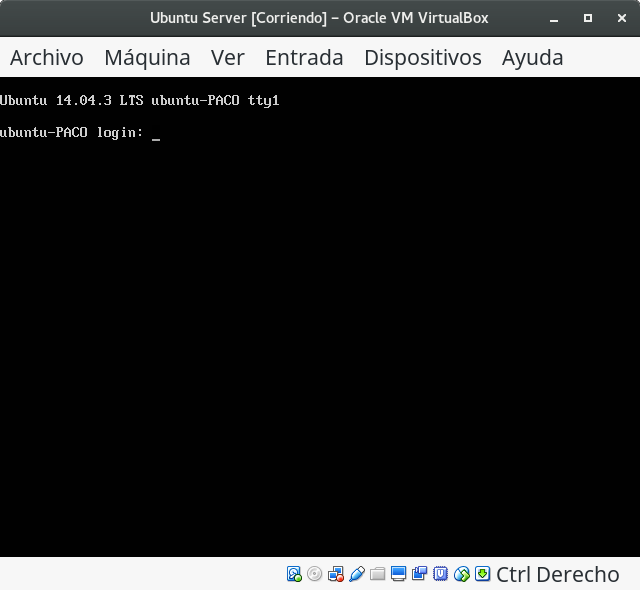
\includegraphics[scale=0.5]{figuras/figura10.png}  %el parámetro scale permite agrandar o achicar la imagen. En el nombre de archivo puede especificar directorios
	
	
	\caption{Podemos observar cómo la máquina sigue arrancando}
	\label{figura10}
\end{figure}

%%%%%%%%%%%%%%%%%%%%%%%%%%%%%%%%%%%%%%%%%%%%%%%%%%%%
% CUESTIÓN 6
%%%%%%%%%%%%%%%%%%%%%%%%%%%%%%%%%%%%%%%%%%%%%%%%%%%%

%Práctica 1
\section{Cuestión opcional 2:}

\subsection{¿Qué relación hay entre los atajos de teclado de emacs y los de la consola bash?}

Los atajos de bash \cite{bash} tienen algunos relación con los de emacs \cite{emacs} ya que la consola de bash se puede poner en modo emacs con el comando \textbf{set -o emacs}. Algunos comandos que se pueden usar serían \cite{emacsmode}: 
\begin{itemize}
	\item ctrl-a	Mover el cursor al comienzo de la línea
	\item ctrl-e	Mover el cursor al final de la línea
	\item meta-b	Mover el cursor una palabra atrás
	\item meta-f	Mover el cursor a la siguiente palabra
	\item ctrl-w	Cortar la última palabra
	\item ctrl-u	Cortar todo lo anterior a donde está el cursor
	\item ctrl-k	Cortar todo lo que hay después del cursor
	\item ctrl-y	Pegar lo último que fue cortado
	\item ctrl-\_	Deshacer
\end{itemize}

\subsection{¿y entre los de vi y las páginas del manual?}

Los comandos de navegación son los mismos en ambos. Por ejemplo, para buscar una palabra se utilizaría el comando /(palabra que quieres buscar). 

%%%%%%%%%%%%%%%%%%%%%%%%%%%%%%%%%%%%%%%%%%%%%%%%%%%%
% CUESTIÓN 7
%%%%%%%%%%%%%%%%%%%%%%%%%%%%%%%%%%%%%%%%%%%%%%%%%%%%

\section{Cuestión opcional 3: Haga lo mismo que con Munin.}

Vamos a utilizar la siguiente demo de Ganglia \cite{ganglia} para enseñar un poco como funciona. Esta demo está basada en los datos que se obtienen de la archiconocida fundación Wikimedia \cite{wikipedia}.\\

La página principal es la que podemos observar en la Figura \ref{figura14}.\\
Ahora, por ejemplo, vamos a ver la carga que ha tenido el grid en la última hora en la Figura \ref{figura15}. Aquí podemos observar:
\begin{itemize}
	\item \textcolor{verde}{Nodes}: no varía el número de nodos que tiene el grid, es constante en esa hora en que se ha estado monitorizando.
	\item \textcolor{rojo}[CPUs]: El número de CPUs es también constante, siendo su valor \textbf{29300 CPUs}.
	\item \textcolor{azuloscuro}{procs}: este si varía siendo el actual valor de procesos 3400, el máximo medido 3900, el mínimo 2500 y la media 3100.
\end{itemize}

Ahora voy a analizar algo que parece también muy interesante que es el uso de la memoria, y podemos observar la cantidad de memoria que se utiliza en una hora en la Figura \ref{figura16}. Los datos que nos muestra:
\begin{itemize}
	\item \textcolor{morado}{Use:} el uso total, el cuál se encuentra en ese momento en 30,9 TB,siendo esta también la media.
	\item \textcolor{azuloscuro}{Share:} uso de memoria compartida, que en esta última hora ha valido 0.
	\item \textcolor{dkgreen}{Cache:} uso de caché, que en el momento actual es de 27,8 TB.
	\item \textcolor{verdelima}{Buffer:} uso del buffer, que en el momento actual es de 856,7 GB.
	\item \textcolor{violeta}{Swap:} uso del swap, que en el momento actual es de 78 TB.
\end{itemize}
\begin{figure}[H] %con el [H] le obligamos a situar aquí la figura
	\centering
	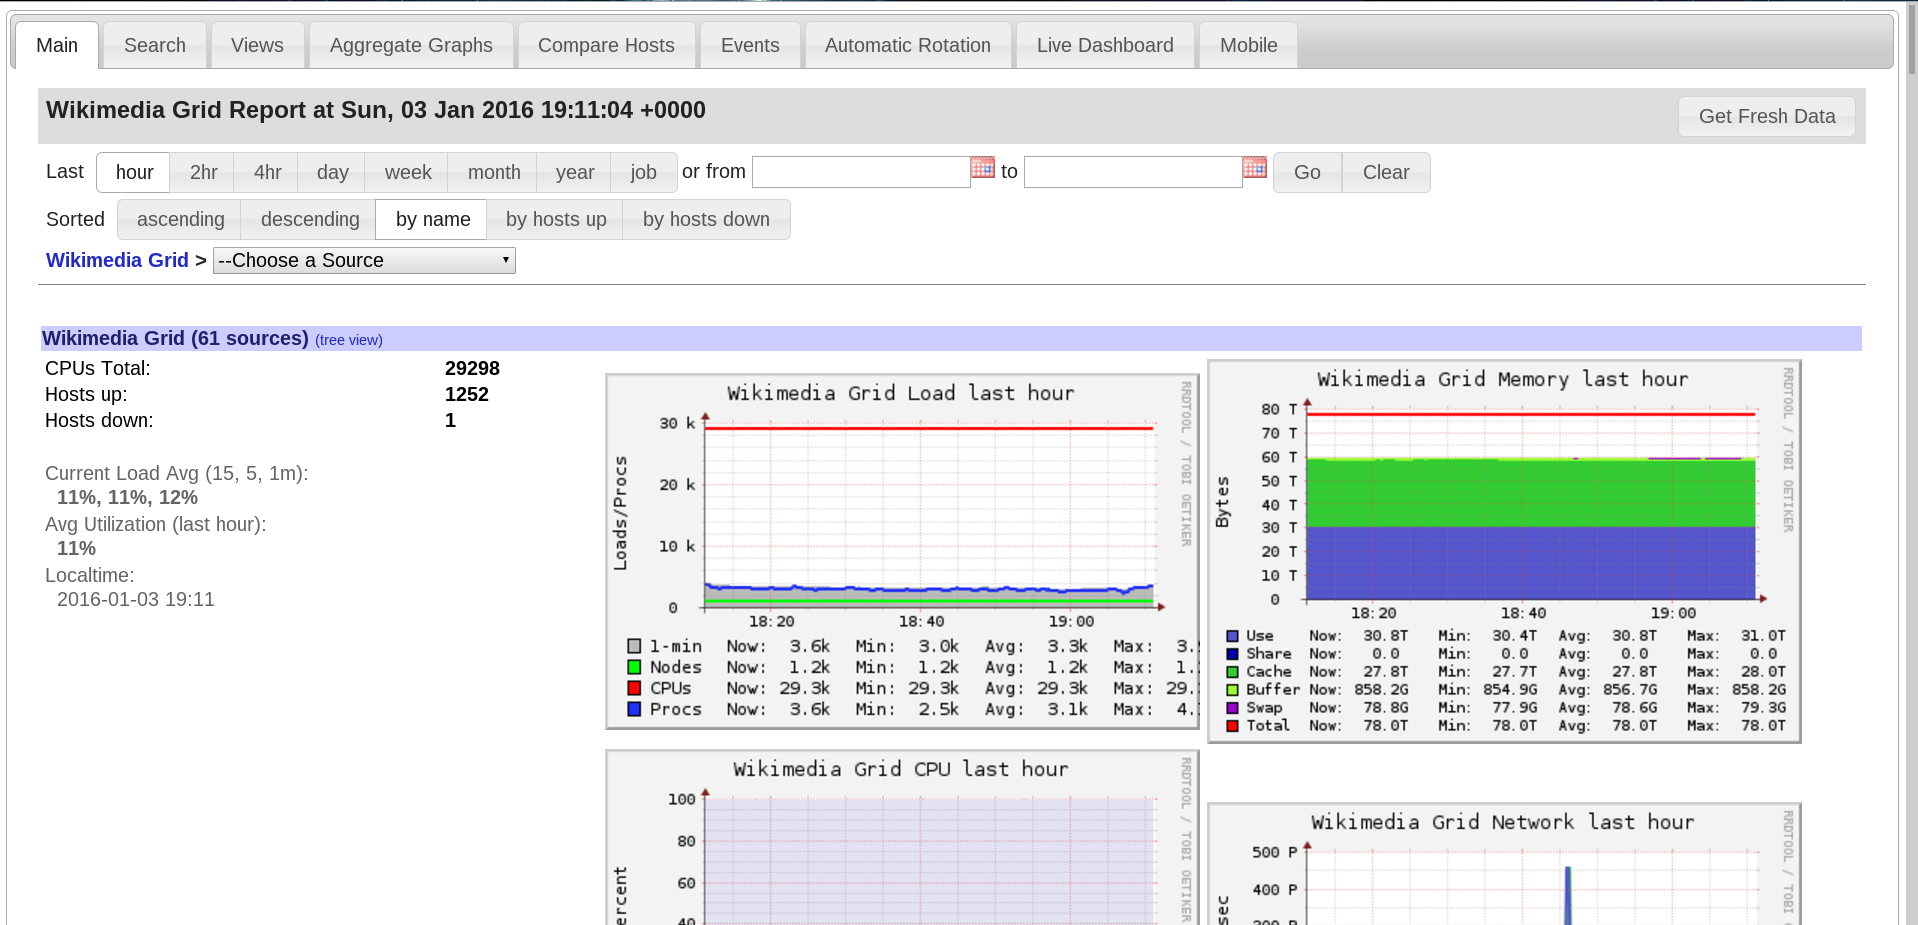
\includegraphics[scale=0.25]{figuras/figura14.png}  %el parámetro scale permite agrandar o achicar la imagen. En el nombre de archivo puede especificar directorios
	
	
	\caption{Página principal de la página demo de Ganglia \cite{ganglia}}
	\label{figura14}
\end{figure}

\begin{figure}[H] %con el [H] le obligamos a situar aquí la figura
	\centering
	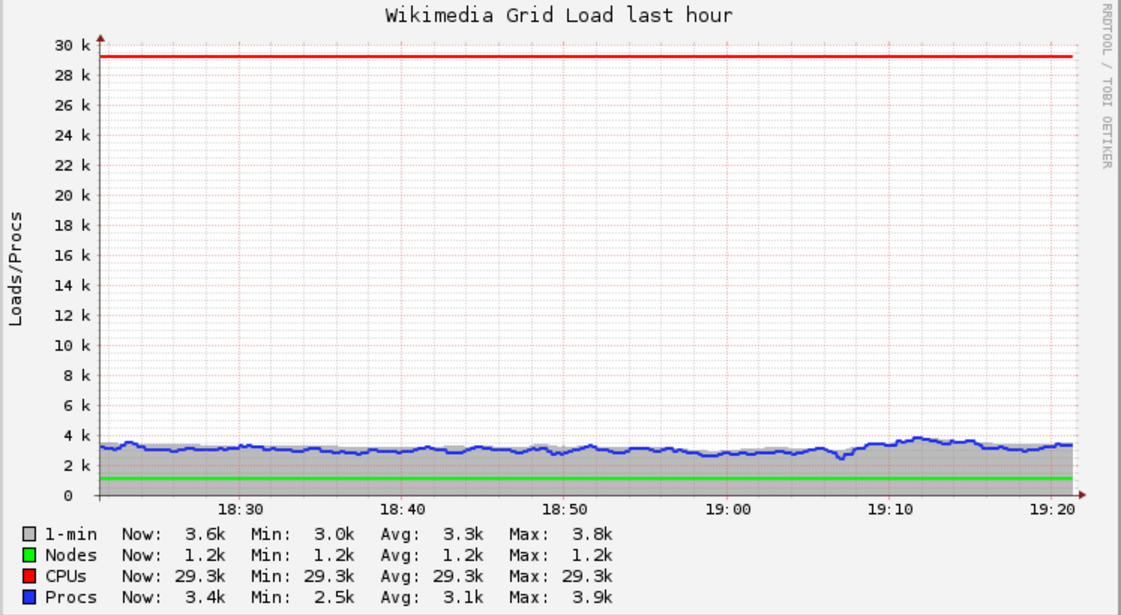
\includegraphics[scale=0.35]{figuras/figura15.png}  %el parámetro scale permite agrandar o achicar la imagen. En el nombre de archivo puede especificar directorios
	
	
	\caption{Carga del grid en la última hora}
	\label{figura15}
\end{figure}
\begin{figure}[H] %con el [H] le obligamos a situar aquí la figura
	\centering
	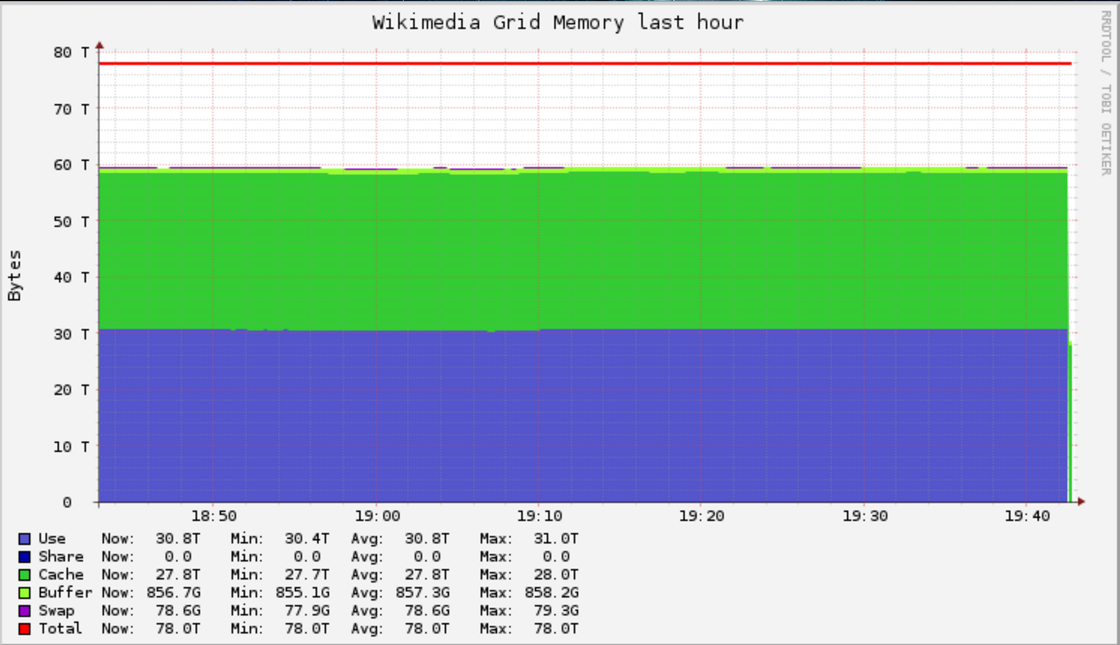
\includegraphics[scale=0.35]{figuras/figura16.png}  %el parámetro scale permite agrandar o achicar la imagen. En el nombre de archivo puede especificar directorios
	
	
	\caption{Uso de memoria en la última hora}
	\label{figura16}
\end{figure}

%%%%%%%%%%%%%%%%%%%%%%%%%%%%%%%%%%%%%%%%%%%%%%%%%%%%
% CUESTIÓN 8
%%%%%%%%%%%%%%%%%%%%%%%%%%%%%%%%%%%%%%%%%%%%%%%%%%%%

%Práctica 4

\section{Cuestión opcional 1: Seleccione, instale y ejecute uno, comente los resultados. Atención: no es lo mismo un benchmark que una suite, instale un benchmark.}

Para listar los test a los que podemos optar utilizamos el comando \textbf{sudo phoronix-test-suite list-available-tests}, y su resultado lo podemos observar en la Figura \ref{figura17}.\\
Ahora vamos a probar a instalar uno cualquiera, por ejemplo \textbf{TSCP}. Para ello utilizamos el comando \textbf{sudo phoronix-test-suite benchmark pts/tscp}, como podemos observar en la Figura \ref{figura18} se empiezan a instalar las dependencias para el benchmark.\\
En la Figura \ref{figura19} podemos observar como nos indica la información de nuestro sistema, y en la Figura \ref{figura20} podemos observar como empieza a correr pero con errores. Cuando termina, Figura \ref{figura21}, vemos que si el tiempo estimado era 4 minutos ha tardado segundos, por lo que podemos indicar que ha encontrado fallos, y nos da al final una puntiación de 79703.

\begin{figure}[H] %con el [H] le obligamos a situar aquí la figura
	\centering
	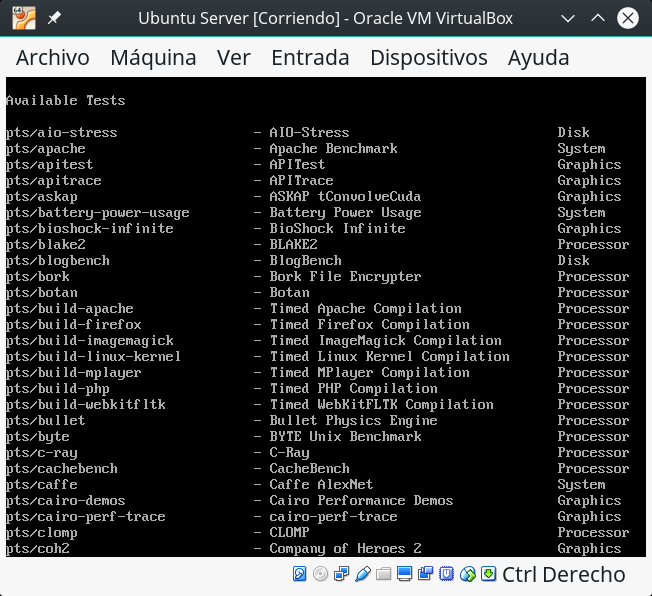
\includegraphics[scale=0.5]{figuras/figura17.png}  %el parámetro scale permite agrandar o achicar la imagen. En el nombre de archivo puede especificar directorios
	
	
	\caption{Resultado de ejecutar el comando \textbf{sudo phoronix-test-suite list-available-tests}}
	\label{figura17}
\end{figure}
\begin{figure}[H] %con el [H] le obligamos a situar aquí la figura
	\centering
	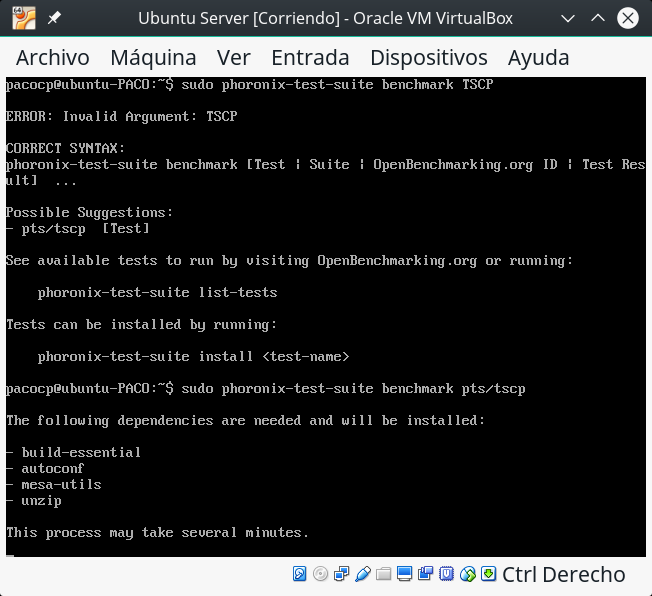
\includegraphics[scale=0.5]{figuras/figura18.png}  %el parámetro scale permite agrandar o achicar la imagen. En el nombre de archivo puede especificar directorios
	
	
	\caption{Se instalan las dependencias para el benchmark}
\label{figura18}
\end{figure}
\begin{figure}[H] %con el [H] le obligamos a situar aquí la figura
	\centering
	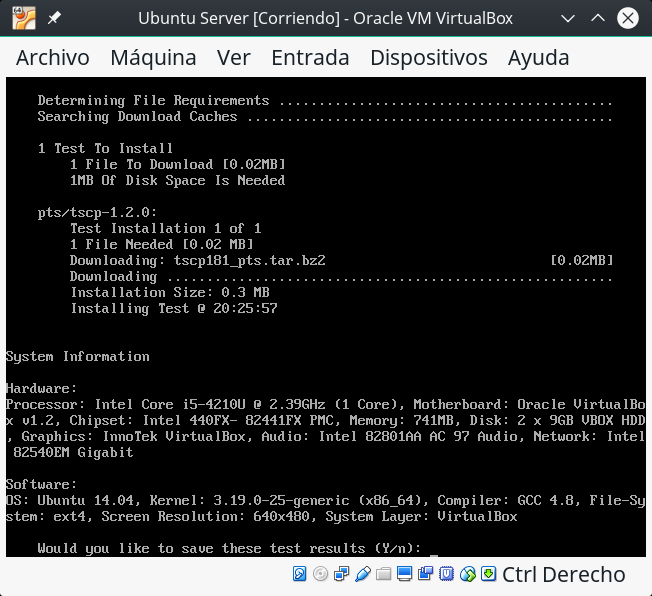
\includegraphics[scale=0.5]{figuras/figura19.png}  %el parámetro scale permite agrandar o achicar la imagen. En el nombre de archivo puede especificar directorios
	
	
	\caption{Vemos como nos dice la información del sistema}
	\label{figura19}
\end{figure}
\begin{figure}[H] %con el [H] le obligamos a situar aquí la figura
	\centering
	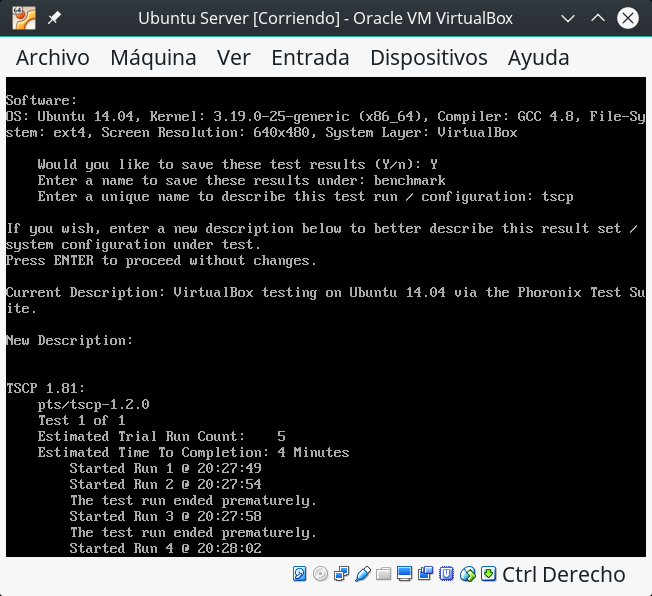
\includegraphics[scale=0.5]{figuras/figura20.png}  %el parámetro scale permite agrandar o achicar la imagen. En el nombre de archivo puede especificar directorios
	
	
	\caption{El benchmark empieza a realizarse}
	\label{figura20}
\end{figure}

\begin{figure}[H] %con el [H] le obligamos a situar aquí la figura
	\centering
	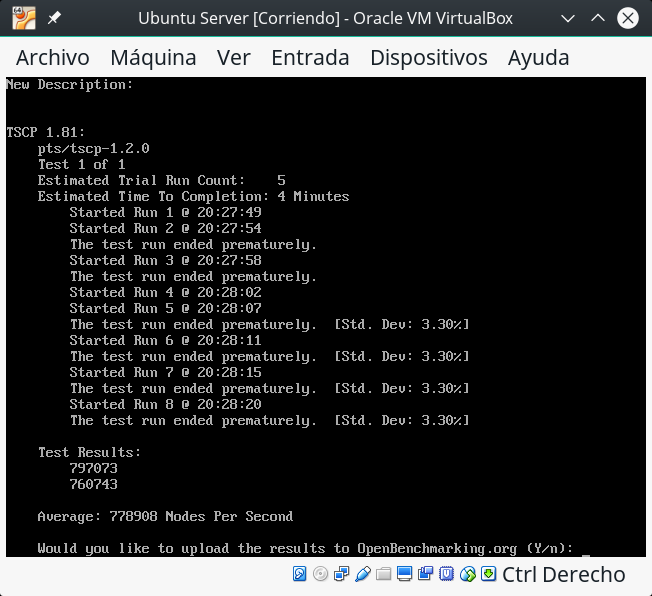
\includegraphics[scale=0.5]{figuras/figura21.png}  %el parámetro scale permite agrandar o achicar la imagen. En el nombre de archivo puede especificar directorios
	
	
	\caption{El benchmark termina con errores y con una puntuación de 79703}
	\label{figura21}
\end{figure}

%%%%%%%%%%%%%%%%%%%%%%%%%%%%%%%%%%%%%%%%%%%%%%%%%%%%
% CUESTIÓN 9
%%%%%%%%%%%%%%%%%%%%%%%%%%%%%%%%%%%%%%%%%%%%%%%%%%%%

\section{Cuestión opcional 7: Desarrolle una página en C o C++ y analice su comportamiento usando valgrind.}

Siguiendo la  página, he cogido el ejemplo de página que lee de un archivo y lo muestra por pantalla. el código es el siguiente:

\begin{lstlisting}[language=C]
#include <stdio.h>
#include <stdlib.h>
#define DATAFILE "data.txt"
int main(void)
{
FILE *f = fopen(DATAFILE,"r");
int ch;
if(f == NULL) {
printf("%s%c%c\n",
"Content-Type:text/html;charset=iso-8859-1",13,10);
printf("<TITLE>Failure</TITLE>\n");
printf("<P><EM>Unable to open data file, sorry!</EM>"); }
else {
printf("%s%c%c\n",
"Content-Type:text/plain;charset=iso-8859-1",13,10);
while((ch=getc(f)) != EOF)
putchar(ch);
fclose(f); }
return 0;
}

\end{lstlisting}

Valgrind lo que realiza es la ejecución del programa y es normalmente usado para saber en que momento del programa desborda la memoria si adolecemos de ese problema. Podemos observar una ejecución sin errores en la Figura \ref{figura22}. También podemos ver una ejecución con fallo en la Figura \ref{figura23}.\\
Podemos observar como en ambos obtienen el mismo resultado, finalizando con la liberación de toda la memoria que estaban usando.
 

\begin{figure}[H] %con el [H] le obligamos a situar aquí la figura
	\centering
	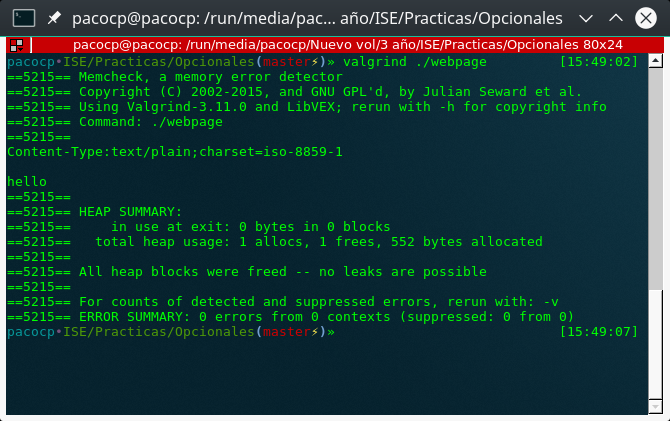
\includegraphics[scale=0.5]{figuras/figura22.png}  %el parámetro scale permite agrandar o achicar la imagen. En el nombre de archivo puede especificar directorios
	
	
	\caption{Ejecución sin errores con Valgrind}
	\label{figura22}
\end{figure}
\begin{figure}[H] %con el [H] le obligamos a situar aquí la figura
	\centering
	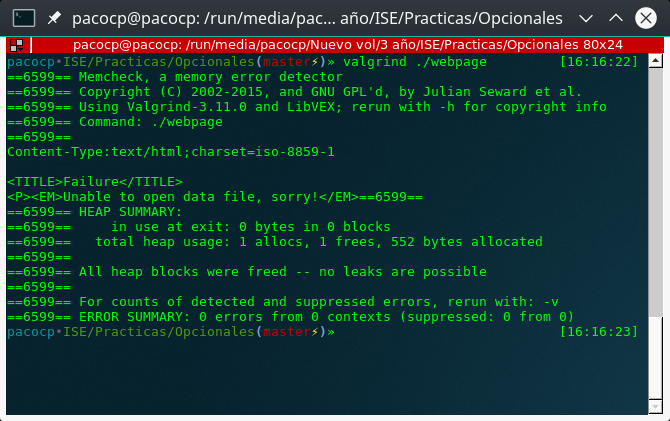
\includegraphics[scale=0.5]{figuras/figura23.png}  %el parámetro scale permite agrandar o achicar la imagen. En el nombre de archivo puede especificar directorios
	
	
	\caption{Ejecución con errores con Valgrind}
	\label{figura23}
\end{figure}

%%%%%%%%%%%%%%%%%%%%%%%%%%%%%%%%%%%%%%%%%%%%%%%%%%%%
% CUESTIÓN 10
%%%%%%%%%%%%%%%%%%%%%%%%%%%%%%%%%%%%%%%%%%%%%%%%%%%%
 %Práctica 2
 
\section{Cuestión opcional 2: Instale y pruebe terminator. Con screen, pruebe su funcionamiento dejando sesiones ssh abiertas en el servidor y recuperándolas posteriomente.}
 
En mi caso para instalar terminator y screen\cite{screen} usamos los comandos: \textbf{sudo pacman -S terminator} y \textbf{sudo pacman -S screen.}\\
Ahora abrimos una sesión de screen, teleando screen y pulsando intro, como podemos observar en la Figura \ref{figura26}, podemos observar el título de la sesión que es screen. Cerramos esa terminal y si la abrimos de nuevo e introducicmos el comando \textbf{screen -r} obtenemos la sesión de screen que teníamos anteriormente, como podemos observar en la Figura \ref{figura27}.
\begin{figure}[H] %con el [H] le obligamos a situar aquí la figura
	\centering
	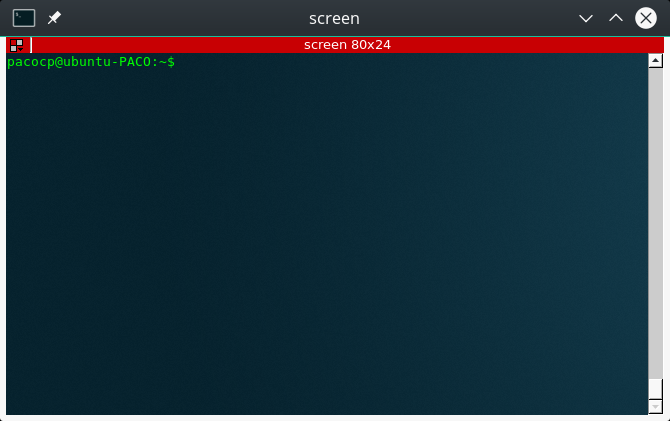
\includegraphics[scale=0.5]{figuras/firgura26.png}  %el parámetro scale permite agrandar o achicar la imagen. En el nombre de archivo puede especificar directorios
	
	
	\caption{Sesión de ssh en screen}
	\label{figura26}
\end{figure}

\begin{figure}[H] %con el [H] le obligamos a situar aquí la figura
	\centering
	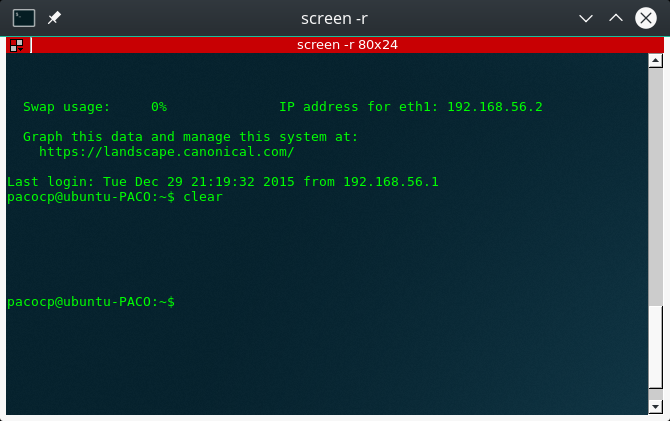
\includegraphics[scale=0.5]{figuras/figura27.png}  %el parámetro scale permite agrandar o achicar la imagen. En el nombre de archivo puede especificar directorios
	
	
	\caption{Recuperamos la sesión de ssh en screen}
	\label{figura27}
\end{figure}

%%%%%%%%%%%%%%%%%%%%%%%%%%%%%%%%%%%%%%%%%%%%%%%%%%%%
% CUESTIÓN 11
%%%%%%%%%%%%%%%%%%%%%%%%%%%%%%%%%%%%%%%%%%%%%%%%%%%%
\section{Cuestión opcional 9: Escriba un script en python y analice su comportamiento usando el profiler presentado.}
El programa sobre el cuál vamos a ejecutar el profiler es el siguiente:\\

\begin{lstlisting}[language=python]
#!/usr/bin/env python
# -*- coding:utf-8 -*-


repeticiones = 100000

for i in range(repeticiones):
valor = (i * 181728712) / 12787
print("El valor es: ")
print(valor)

\end{lstlisting}

Voy a utilizar el \textbf{CProfile} \cite{pprofiler} para analizar el programa, para ello utilizamos el siguiente comando:\\
\textbf{python -m cProfile  -s 'name'  profiler.py}\\

La opción -s 'name' sirve para ordenarlo por nombre.\\
Y obtenemos el siguiente resultado:\\

\begin{figure}[H] %con el [H] le obligamos a situar aquí la figura
	\centering
	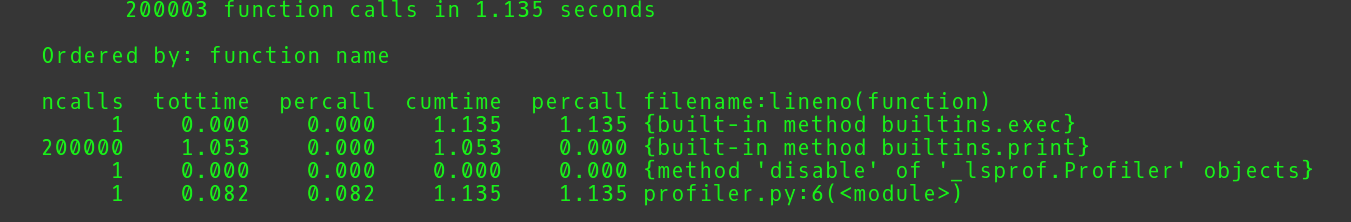
\includegraphics[scale=0.35]{figuras/figura30.png}  %el parámetro scale permite agrandar o achicar la imagen. En el nombre de archivo puede especificar directorios
	\label{figura30}
	
	\caption{Resultados del profiler} 
\end{figure}

Podemos observar que nos encontramos lo primero con el número de llamadas totales y el tiempo de ejecución del programa. En este caso son 200003 llamadas a funciones en 1.135 segundos.\\
Luego nos indica cómo se encuentran ordenada la información que nos muestra, en este caso es por nombre, ya que es como le he indicado anteriormente.\\
Ahora nos encontramos con 6 columnas:
\begin{itemize}
	\item \textbf{ncalls: } número de veces que se llama a la función. En nuestro caso, la primera función que es la \textbf{ejecución} solo se la llama una vez, ya que es la ejecución. La segunda función es \textbf{print} que se le llama 200000, que es el número de veces que itera el bucle for. Y la llamada al \textbf{programa} profiler.py .
	\item \textbf{tottime: } que es el tiempo interno. En este caso sólo tienen valor la llamada a la función \textbf{print} y la llamada al \textbf{programa} .
	\item \textbf{percall: } por llamada. El único campo con valor es el del \textbf{programa}
	\item \textbf{cumtime: } tiempo acumulativo que es el tiempo en total de todas las llamadas de una función. En este caso los valores de la función de \textbf{ejecución} y la de la llamada al \textbf{programa} son los mismos y estos son iguales al valor total del tiempo de funcionamiento del programa. Podemos observar como el otro campo que tiene valor es el de la función \textbf{print}  que vale 1.053, un valor menor al de tiempo total de ejecución.
	\item \textbf{percall: } de nuevo el tiempo por llamada pero esta vez respecto al cumtime.
\end{itemize}

%%%%%%%%%%%%%%%%%%%%%%%%%%%%%%%%%%%%%%%%%%%%%%%%%%%%
% CUESTIÓN 12
%%%%%%%%%%%%%%%%%%%%%%%%%%%%%%%%%%%%%%%%%%%%%%%%%%%%

\section{Cuestión opcional 1: Indique qué comandos ha utilizado para realizarlo así como capturas de pantalla del proceso de reconstrucción del RAID.}

Para realizar este procedimiento he usado el recurso dado en la pregunta opcional 1 de la práctica 1 \cite{raid}.

\begin{figure}[H] %con el [H] le obligamos a situar aquí la figura
	\centering
	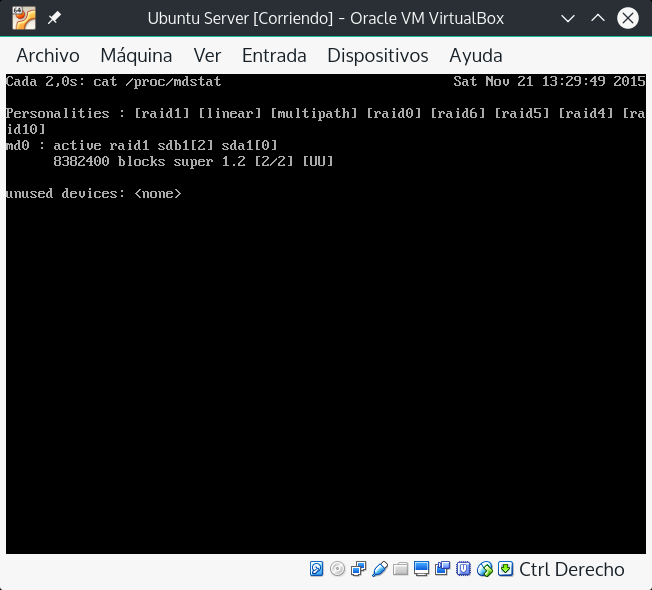
\includegraphics[scale=0.5]{figuras/figura32.png}  %el parámetro scale permite agrandar o achicar la imagen. En el nombre de archivo puede especificar directorios
	\label{figura32}
	
	\caption{Podemos observar cómo tenemos 2 RAID en uso con el comando: \textbf{watch -n2 cat /proc/mdstat}} 
\end{figure}

\begin{figure}[H] %con el [H] le obligamos a situar aquí la figura
	\centering
	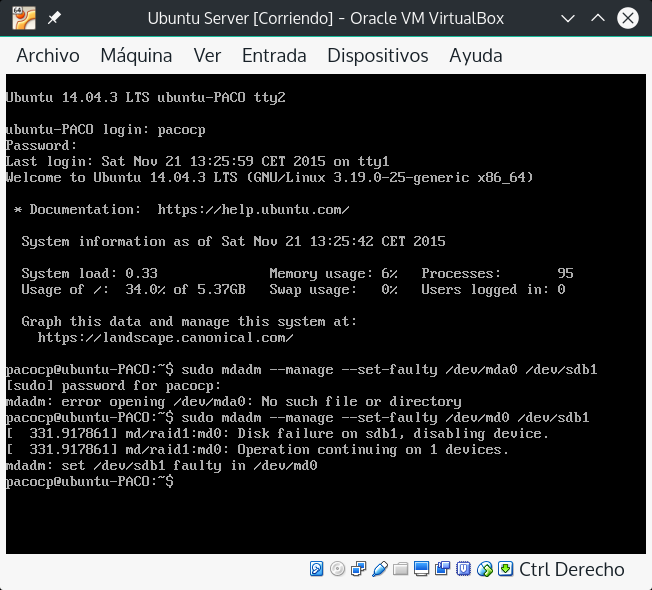
\includegraphics[scale=0.5]{figuras/figura33.png}  %el parámetro scale permite agrandar o achicar la imagen. En el nombre de archivo puede especificar directorios
	\label{figura33}
	
	\caption{Usando el comando \textbf{sudo mdadm --manage --set-faulty /dev/md0 /dev/sdb1} para indicarle que ponga en fallo a sdb1} 
\end{figure}


\begin{figure}[H] %con el [H] le obligamos a situar aquí la figura
	\centering
	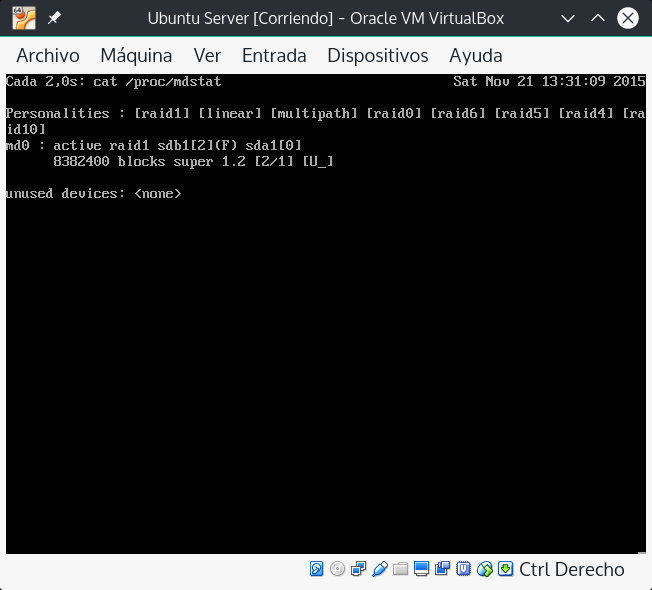
\includegraphics[scale=0.5]{figuras/figura34.png}  %el parámetro scale permite agrandar o achicar la imagen. En el nombre de archivo puede especificar directorios
	\label{figura34}
	
	\caption{Podemos observar cómo ahora en la terminal del watch sólo nos salen 2/1} 
\end{figure}

\begin{figure}[H] %con el [H] le obligamos a situar aquí la figura
	\centering
	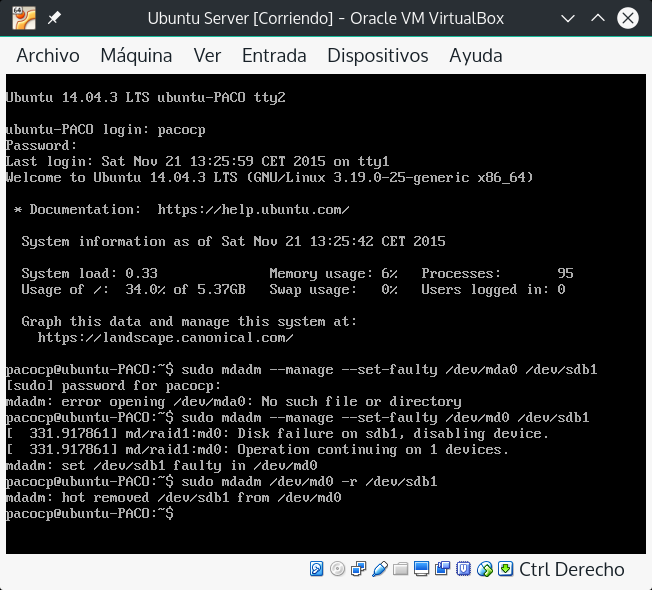
\includegraphics[scale=0.5]{figuras/figura35.png}  %el parámetro scale permite agrandar o achicar la imagen. En el nombre de archivo puede especificar directorios
	\label{figura35}
	
	\caption{Con el comando \textbf{sudo mdadm /dev/md0 -r /dev/sdb1} eliminamos a sdb1} 
\end{figure}

\begin{figure}[H] %con el [H] le obligamos a situar aquí la figura
	\centering
	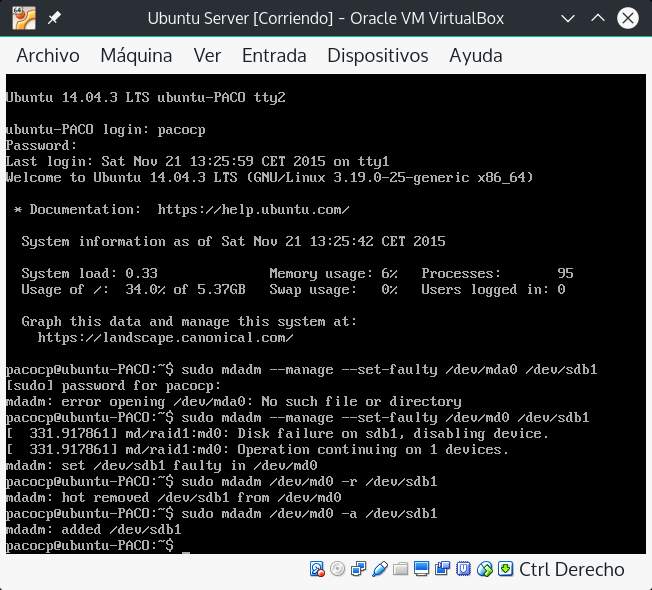
\includegraphics[scale=0.5]{figuras/figura36.png}  %el parámetro scale permite agrandar o achicar la imagen. En el nombre de archivo puede especificar directorios
	\label{figura36}
	
	\caption{Con el comando \textbf{sudo mdadm /dev/md0 -a /dev/sdb1} añadimos de nuevo sdb1} 
\end{figure}

\begin{figure}[H] %con el [H] le obligamos a situar aquí la figura
	\centering
	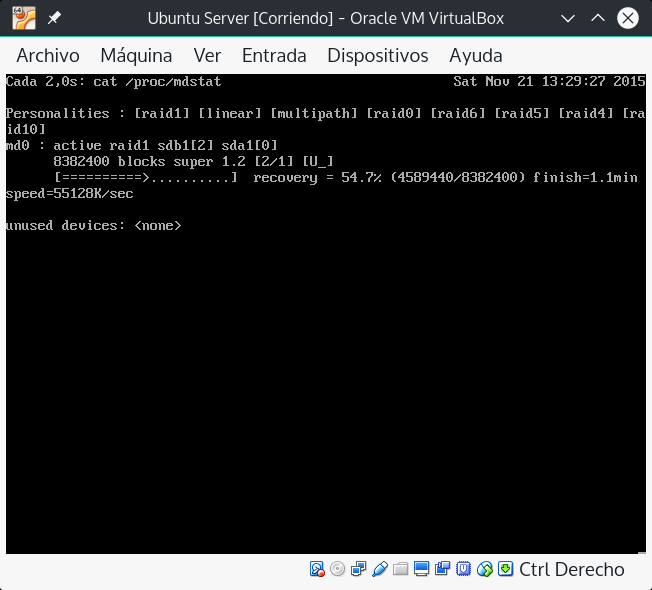
\includegraphics[scale=0.5]{figuras/figura31.png}  %el parámetro scale permite agrandar o achicar la imagen. En el nombre de archivo puede especificar directorios
	\label{figura31}
	
	\caption{Y si nos desplazamos a la terminal com el watch podemos observar como está recuperando el disco} 
\end{figure}
\newpage
\bibliography{citas} %archivo citas.bib que contiene las entradas 
\bibliographystyle{ieeetr} % hay varias formas de citar
\end{document}